\section{Voraussetzungen}

\subsection{Versuchsziel}

Ziel des Versuches zum Compton-Effekt ist die Bestimmung des totalen
Compton-Wirkungsquerschnitts für $^{137}$Cs. Um dies zu erreichen wird ein
Aluminium-Block mit hochenergetischen Photonen aus radioaktiven Präparate
beschossen. Die gestreuten Photonen werden schließlich ihrer Energie nach
computergestützt vermessen.

\subsection{Physikalische Grundlagen}

Das Photon kann auf drei verschiedene Arten mit Atomen wechselwirken:
\begin{enumerate}[i)]
  \item Photoelektrischer Effekt
  \item Compton-Effekt
  \item Paarbildung
\end{enumerate}
Welcher Prozess im Einzelfall statt findet, hängt im Wesentlichen von der
Energie ab. Der photoelektrische Effekt dominiert bei Energien bis hin zu
einigen Hundert \si{\kilo\eV}. Da bei Paarbildung die Energie für die Masse des
Elektron-Antielektron-Paar bereitgestellt werden muss, findet dieser Prozess
erst ab einer Photonenenergie über \SI{5}{\mega\eV} statt.

Zwischen diesen Grenzen dominiert der Compton-Effekt. Hierbei wird das Photon
inelastisch an einem Hüllenelektron des Atoms gestreut. Der differentielle
Wirkungsquerschnitt $\frac{\dd{σ}}{\dd{\Omega}}$, wie in \cite[Gl. 1]{script}
beschrieben, ist abhängig von der Energie des Photons vor dem Stoß $E_0$ und
nach dem Stoß $E'$ und dem Ablenkwinkel θ.
\begin{equation}
  \frac{\dd{σ}}{\dd{\Omega}} = \frac{r_0^2}{2}κ^2\left(\frac{1}{κ}+\frac{κ}{1}-\sin^2\theta\right)
  \,
  \mathrm{mit}
  \,
  κ = \frac{E'}{E_0}
  \label{eqn:diff_sigma}
\end{equation}

\subsection{Versuchsaufbau}

Der totale Wirkungsquerschnitt σ, der theoretisch über das Raumintegral von
\eref{diff_sigma} beschrieben wird, lässt sich auch experimentell messen.
\begin{figure}[htb]
      \centering
      \includegraphics[page=6,width=1\columnwidth,keepaspectratio,viewport=81 397 504 635,clip,]{../docs/compton}
      \caption{Schema des Versuchsaufbaus}
      \label{fig:aufbau}
\end{figure}

Wie der \fref{aufbau} zu entnehmen ist, werden die hochenergetischen Photonen
, die in Folge des radioaktiven Zerfalls der Probe entstehen, kolliminiert und
durch einen massiven Aluminiumblock geleitet. Durch die sich anschließende
auf Szintillatore basierende Messtechnik werden die einzelnen Photonen ihrer
Energie nach registriert. Durch die Verwendung von Photomultipliern und
Messverstärkern kann das Signal schließlich digital mit dem PC aufgezeichnet
werden. Doch bevor diese eigentliche Messung stattfinden kann, sind noch einige
andere Messungen nötig.

Als ersten muss das Hintergrundrauschen vermessen werden. Hierzu wird der
Aluminiumblock entfernt und eine Stunde lang gemessen, welche Strahlung auch
ohne radioaktive Probe vorhanden ist.

Anschließend muss die Messvorrichtung geeicht werden. Hierfür werden radioaktive
Isotope mit γ-Strahlung unterschiedlicher Energien verwendet.

Weiterhin ist auch eine Vergleichsmessung mit radioaktiver Probe, aber ohne
Aluminiumblock, nötig.

Alle Messungen werden auf die jeweilige Öffnungszeit (Messzeit abzüglich Totzeit)
des Messapparats normiert.

\subsection{Verwendete Geräte}

Für die Versuchsdurchführung wurde der im \cite{script} vorgeschlagenen und
bereits vorbereitete Aufbau verwendet. Eine Auflistung aller verwendeten
Geräte und Materialien befindet sich ebenfalls im \cite[Kap. 6]{script}.